\transition{Object Serialization Using PUP: The Pack/UnPack Framework}

\begin{frame}[fragile]
\frametitle{The PUP Process}
  \begin{center}
    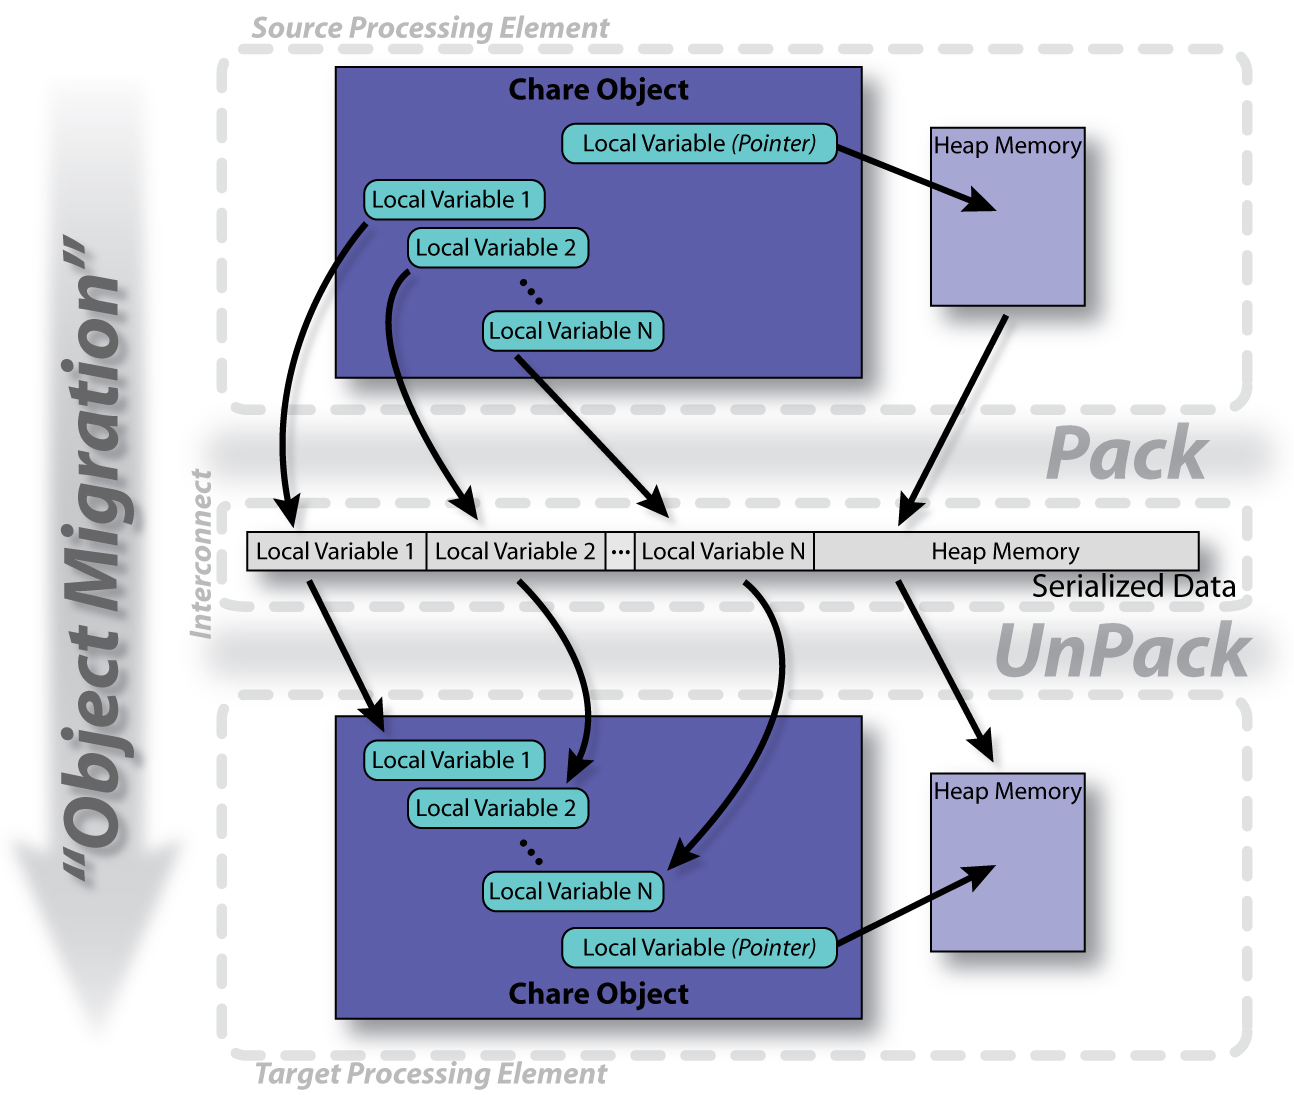
\includegraphics[width=0.8\textwidth]{figures/PUPProcess.png}
  \end{center}
\end{frame}

%for class
\begin{frame}[fragile]
\frametitle{PUP Usage Sequence}
  \begin{center}
    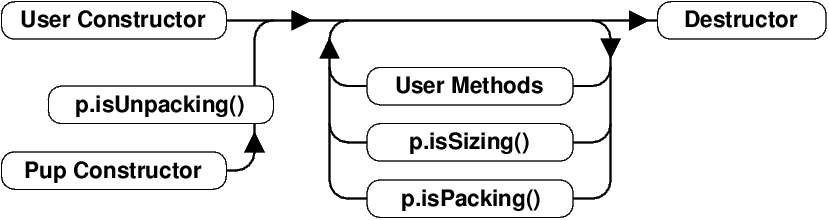
\includegraphics[width=0.8\textwidth]{figures/PUPUsage.png}
  \end{center}
\begin{columns}
 \begin{column}{0.5\textwidth}
 \begin{itemize}
 \item Migration out:
   \begin{itemize}
    \item ckAboutToMigrate
    \item Sizing
    \item Packing
    \item Destructor
    \end{itemize}
 \end{itemize}
 \end{column}

 \begin{column}{0.5\textwidth}
 \begin{itemize}
    \item Migration in:
    \begin{itemize}
    \item Migration constructor
    \item UnPacking
    \item ckJustMigrated
    \end{itemize}
  \end{itemize}
\end{column}

\end{columns}
\end{frame}
%\end for class 

\begin{frame}[fragile]
\frametitle{Writing a PUP routine}
 \begin{columns}
 \begin{column}{0.5\textwidth}
   \begin{lstlisting}
class MyChare : public CBase_MyChare {
  int a;
  float b;
  char c;
  float localArray[LOCAL_SIZE];
};
 \end{lstlisting}
 \end{column}
 \begin{column}{0.5\textwidth}
  \begin{lstlisting}
void pup(PUP::er &p) {
   CBase_MyChare::pup(p);
   p | a;
   p | b;
   p | c;
   p(localArray, LOCAL_SIZE);
}
  \end{lstlisting}
  \end{column}
  \end{columns}
\end{frame}

\begin{frame}[fragile]
\frametitle{Writing a PUP routine}
 \begin{columns}
 \begin{column}{0.5\textwidth}
   \begin{lstlisting}
class MyChare : public CBase_MyChare {
  int heapArraySize;
  float* heapArray;
  MyClass *pointer;
};
 \end{lstlisting}
 \end{column}
 \begin{column}{0.5\textwidth}
  \begin{lstlisting}
void pup(PUP::er &p) {
   CBase_MyChare::pup(p);
   p | heapArraySize;
   if (p.isUnpacking()) {
     heapArray = new float[heapArraySize];
   }
   p(heapArray, heapArraySize);
   bool isNull = !pointer;
   p | isNull;
   if (!isNull) {
     if (p.isUnpacking()) pointer = new MyClass();
     p | *pointer;
   }
 }
}
  \end{lstlisting}
  \end{column}
  \end{columns}
\end{frame}


\begin{frame}[fragile]
\frametitle{PUP: Concerns}
\begin{itemize}
\item If variables are added to an object, update the PUP routine
\item If the object allocates data on the heap, copy it recursively, not just the pointer
\item Remember to allocate memory while unpacking
\item Sizing, Packing, and Unpacking must scan the variables in the same order
\item Test PUP routines with “+balancer RotateLB”
\end{itemize}
\end{frame}
